\input{SlideInclude.tex}

\title[Empirical application]{Empirical Applications of the Solow Model}


\begin{document}
\maketitle

\section{Transitional growth}

\begin{frame}{Germany after WWII}
\begin{center}
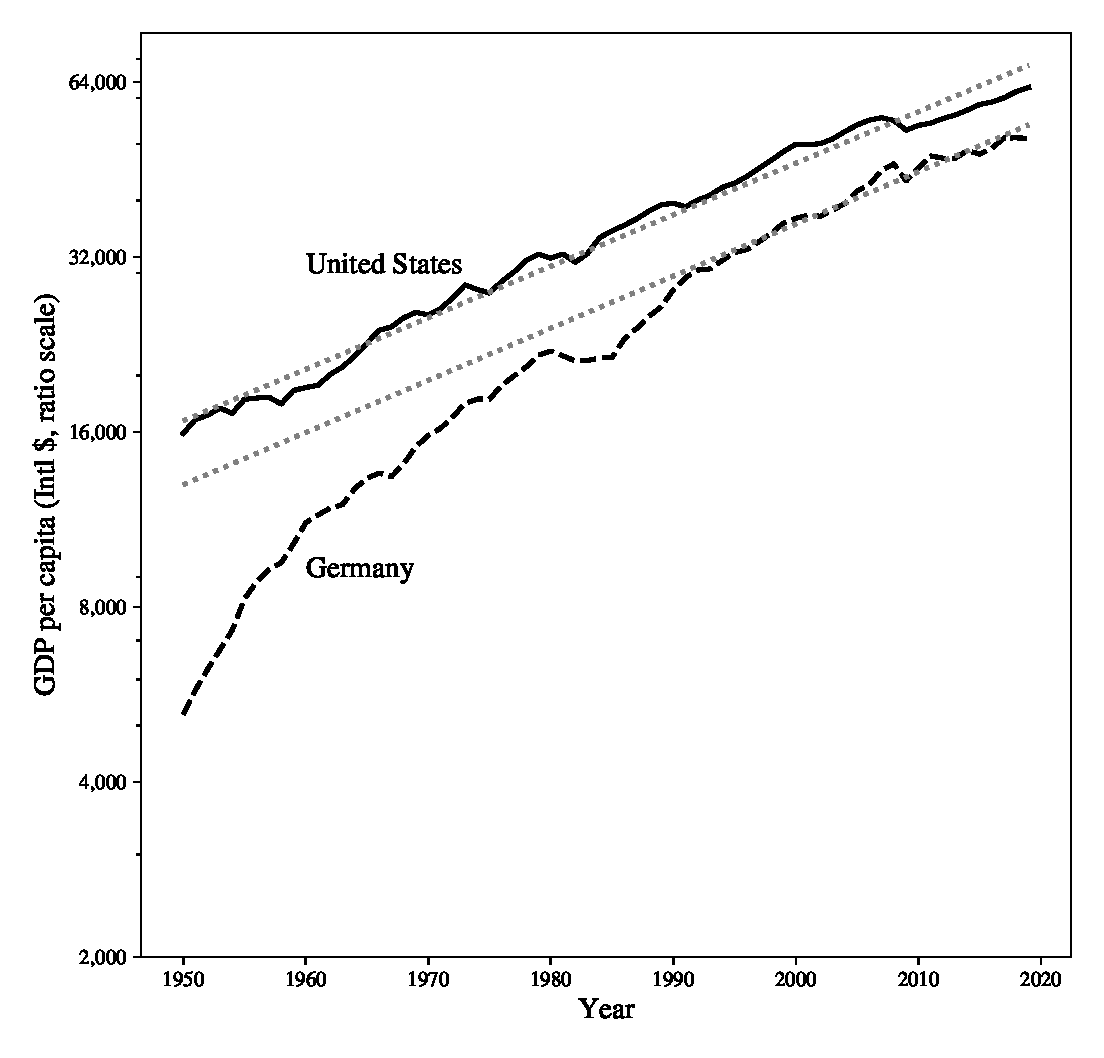
\includegraphics[height = 3in]{../Figures/fig-ch3-fig1.eps}
\end{center}
\end{frame}

\begin{frame}{Germany after WWII}
The data from Germany is consistent with:
\begin{itemize}
	\item A substantial loss of $K$ in the war relative to $L$
	\item The ``initial'' $K/AL$ ratio in 1946 is very low and below steady state
	\item The dynamics of capital imply a high $g_K$
	\item Transitional growth $\alpha(g_K - g_A - g_L)$ is very high for a time
	\item Transitional growth dissipates as Germany reaches the BGP
	\item Germany's BGP is lower than the US, so there remains some difference in parameters ($s_I$, $A_0$, $g_L$) creating a level difference
\end{itemize}
\end{frame}

\begin{frame}{South Korea and China}
\begin{center}
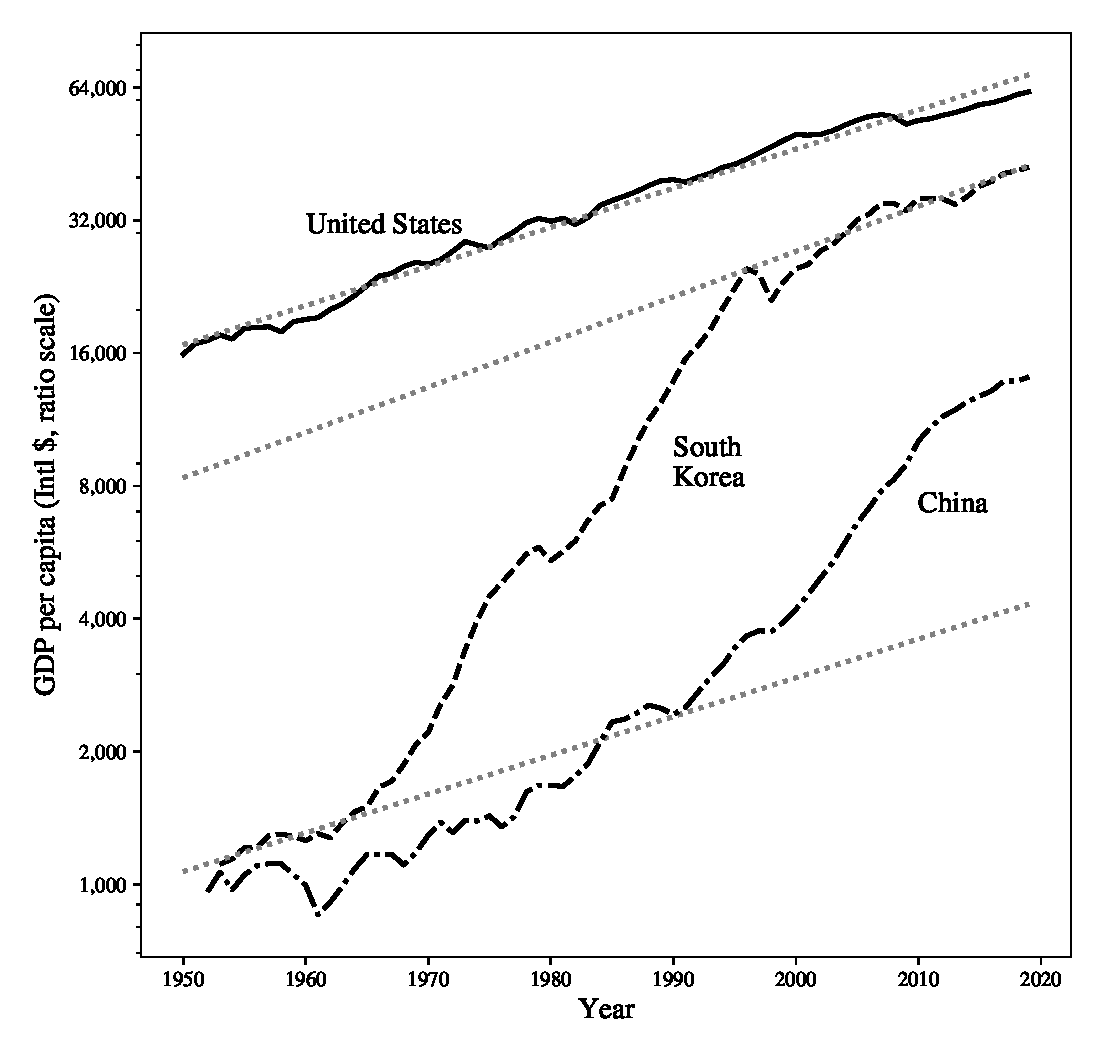
\includegraphics[height = 3in]{../Figures/fig-ch3-fig2.eps}
\end{center}
\end{frame}

\begin{frame}{South Korea and China}
The data from East Asia is consistent with:
\begin{itemize}
	\item South Korea and China are on a ``low'' BGP in the 1950s and 1960s 
	\item Around 1970 something shifts the S. Korea BGP up
	\item South Korea's $K/AL$ is thus below steady state around 1970
	\item Transitional growth occurs because $\alpha(g_K - g_A - g_L)$ is positive
	\item By 2000 South Korea has converged to new BGP and growth rate matches that in the US
	\item Around 1990 something shifts the Chinese BGP up and $K/AL$ is below steady state
	\item Transitional growth is occurring in China, but we don't quite know if it has reached the enw BGP yet.
\end{itemize}
\end{frame}

\begin{frame}{What changed the East Asian BGP?}
\begin{center}
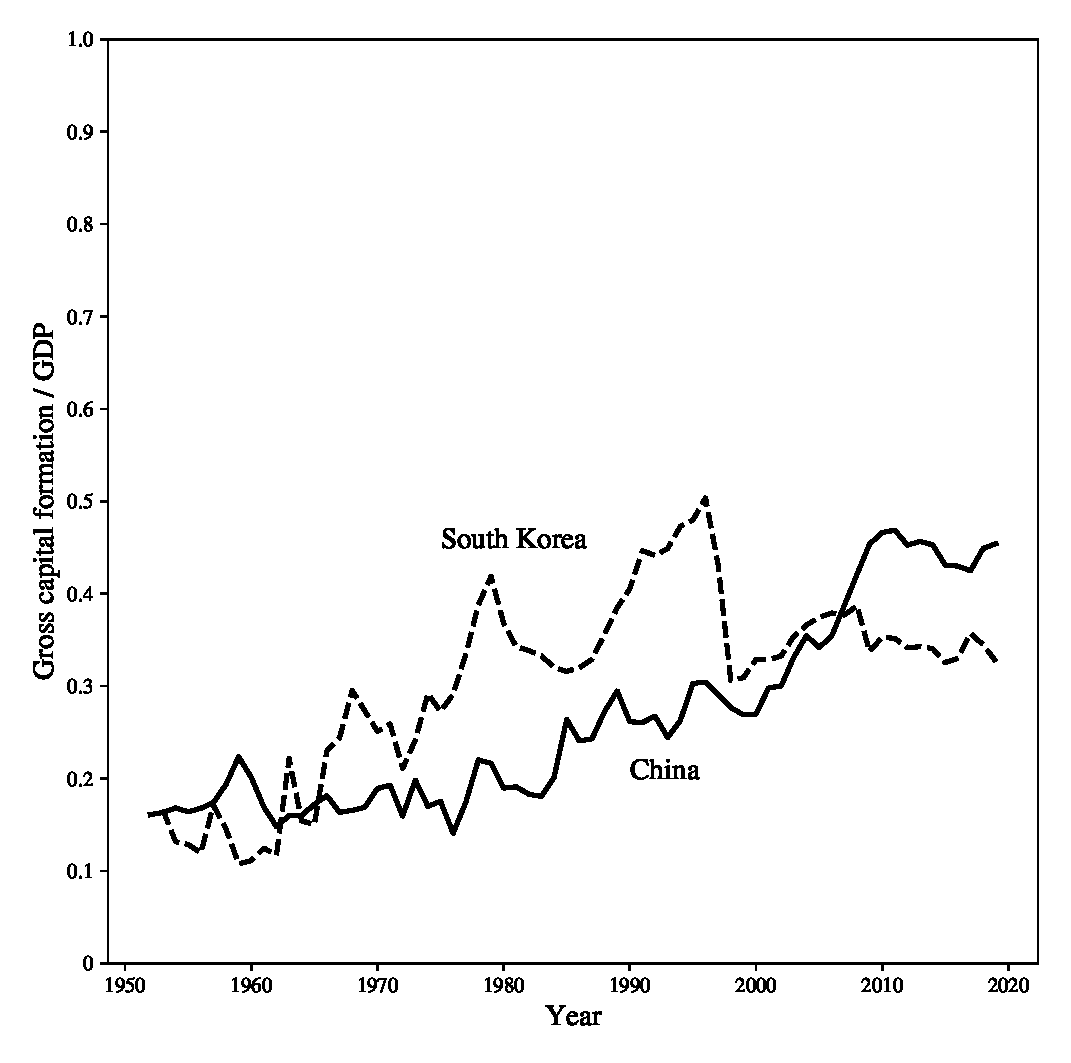
\includegraphics[height = 3in]{../Figures/fig-ch3-fig3.eps}
\end{center}
\end{frame}

\begin{frame}{What changed the East Asian BGP?}
\begin{center}
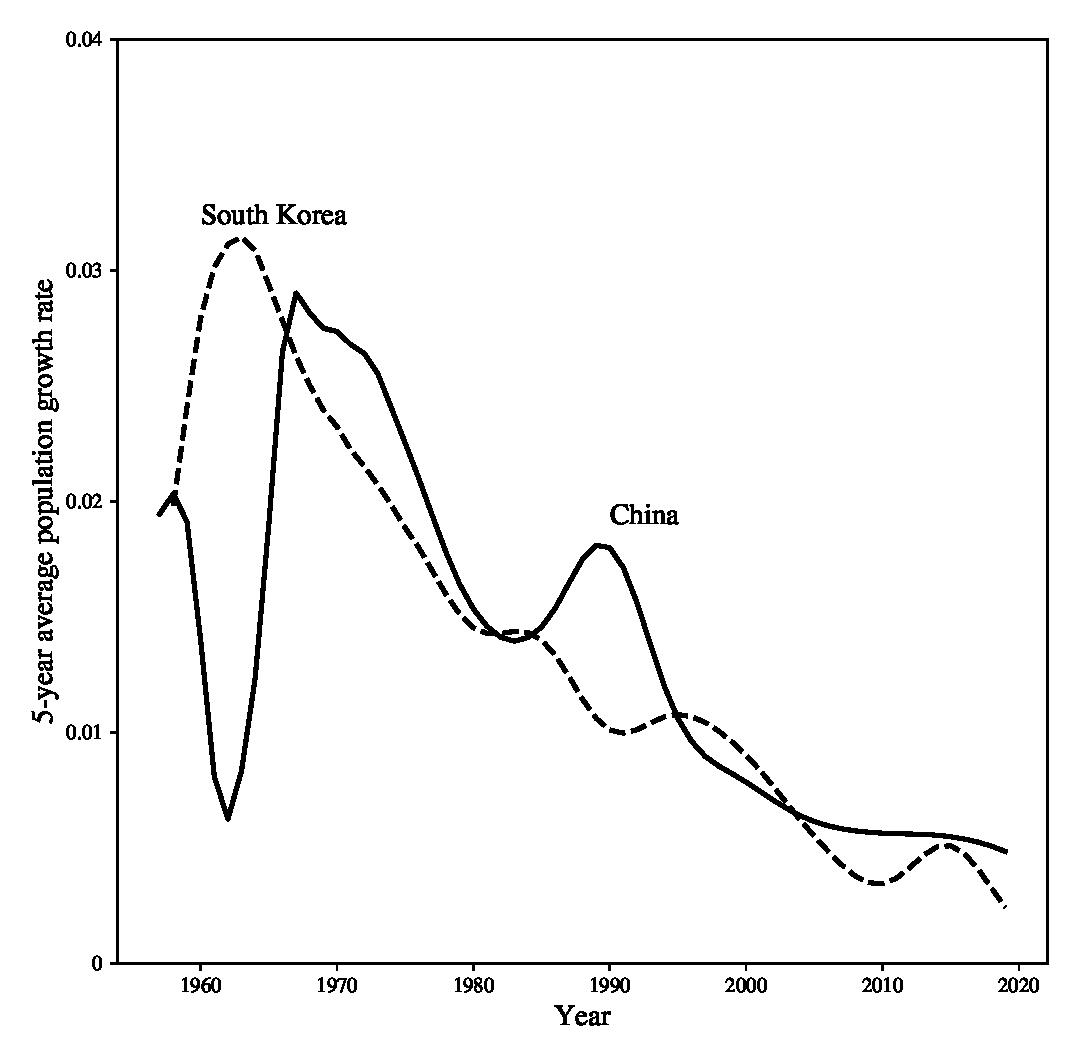
\includegraphics[height = 3in]{../Figures/fig-ch3-fig4.eps}
\end{center}
\end{frame}

\section{Cross-section}
\begin{frame}{Differences in levels}
Remember the level of GDP per capita on the BGP is
\begin{equation}
	\log y_t^{BGP} = \underset{\text{Intercept}}{\left(\frac{\alpha}{1-\alpha} \log \left(\frac{s_I}{g_A + g_L + \delta} \right) + \log A_0\right)} + \underset{\text{Slope}}{g_A} t. \nonumber
\end{equation}
so that the intercept tells us about differences in levels of GDP per capita, even if the growth rate (slope) is the same.
\begin{itemize}
	\item All else equal, a higher $s_I$ should imply a higher level of GDP per capita
	\item All else equal, a lower $g_L$ should imply a higher level of GDP per capita
\end{itemize}
Other parameters matter but are harder to measure.
\end{frame}

\begin{frame}{Levels and capital formation rates}
\begin{center}
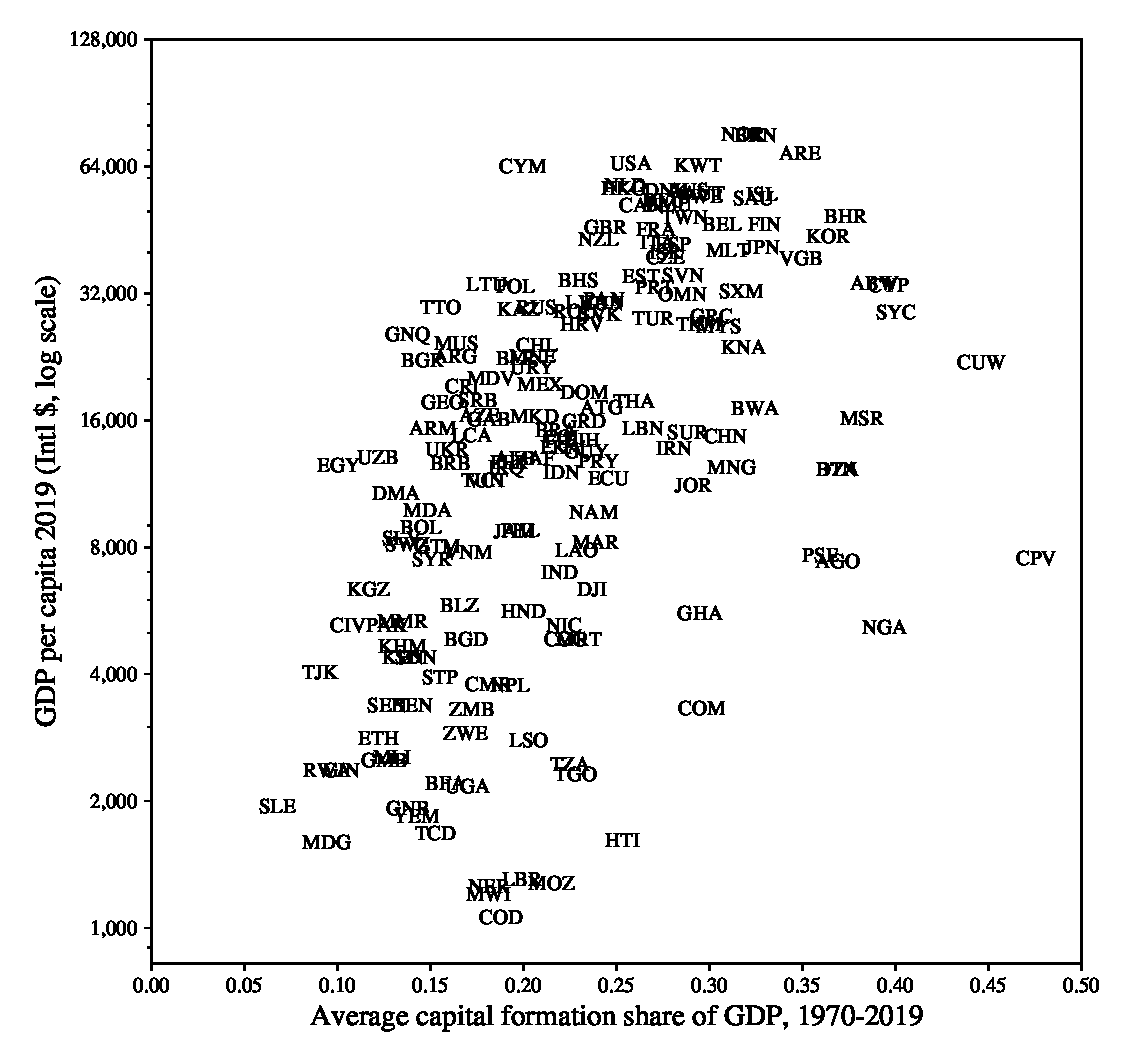
\includegraphics[height = 3in]{../Figures/fig-ch3-fig5.eps}
\end{center}
\end{frame}

\begin{frame}{Levels and population growth rates}
\begin{center}
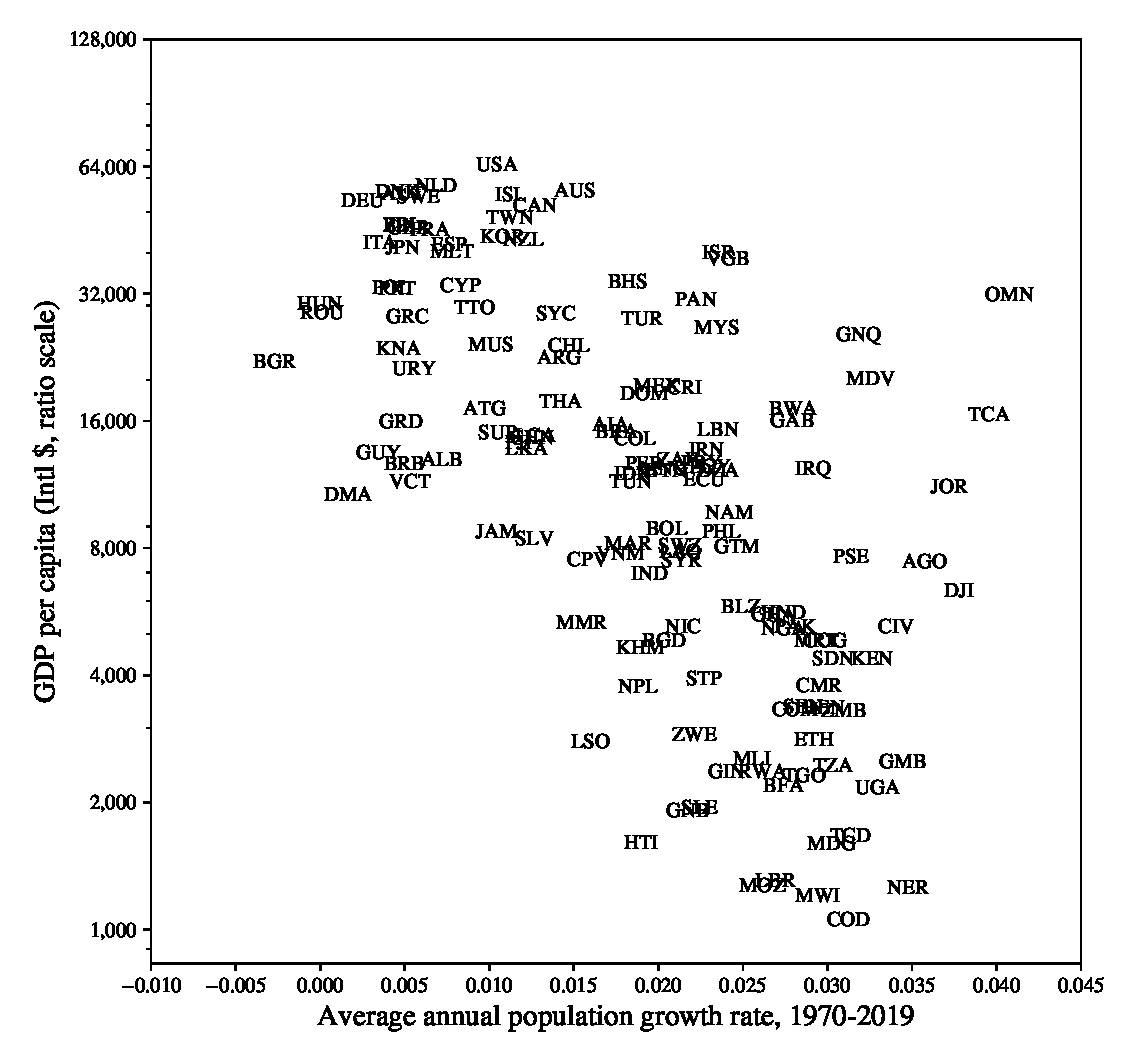
\includegraphics[height = 3in]{../Figures/fig-ch3-fig6.eps}
\end{center}
\end{frame}

\section{Convergence}
\begin{frame}{Growth rates an initital levels}
If the \textit{only} thing that differed across countries was initial $K_0/A_0L_0$, then:
\begin{itemize}
	\item Countries with low $K_0/A_0 L_0$ would have a low \textit{level} of GDP per capita
	\item Countries with low $K_0/A_0 L_0$ would have a high growth rate of GDP per capita because of transitional growth
	\item So we'd expect to see that growth rates were negatively related to the level of GDP per capita
\end{itemize}
\end{frame}

\begin{frame}{Convergence in rich countries}
This is for a set of currently rich countries from 1870 to 2018
\begin{center}
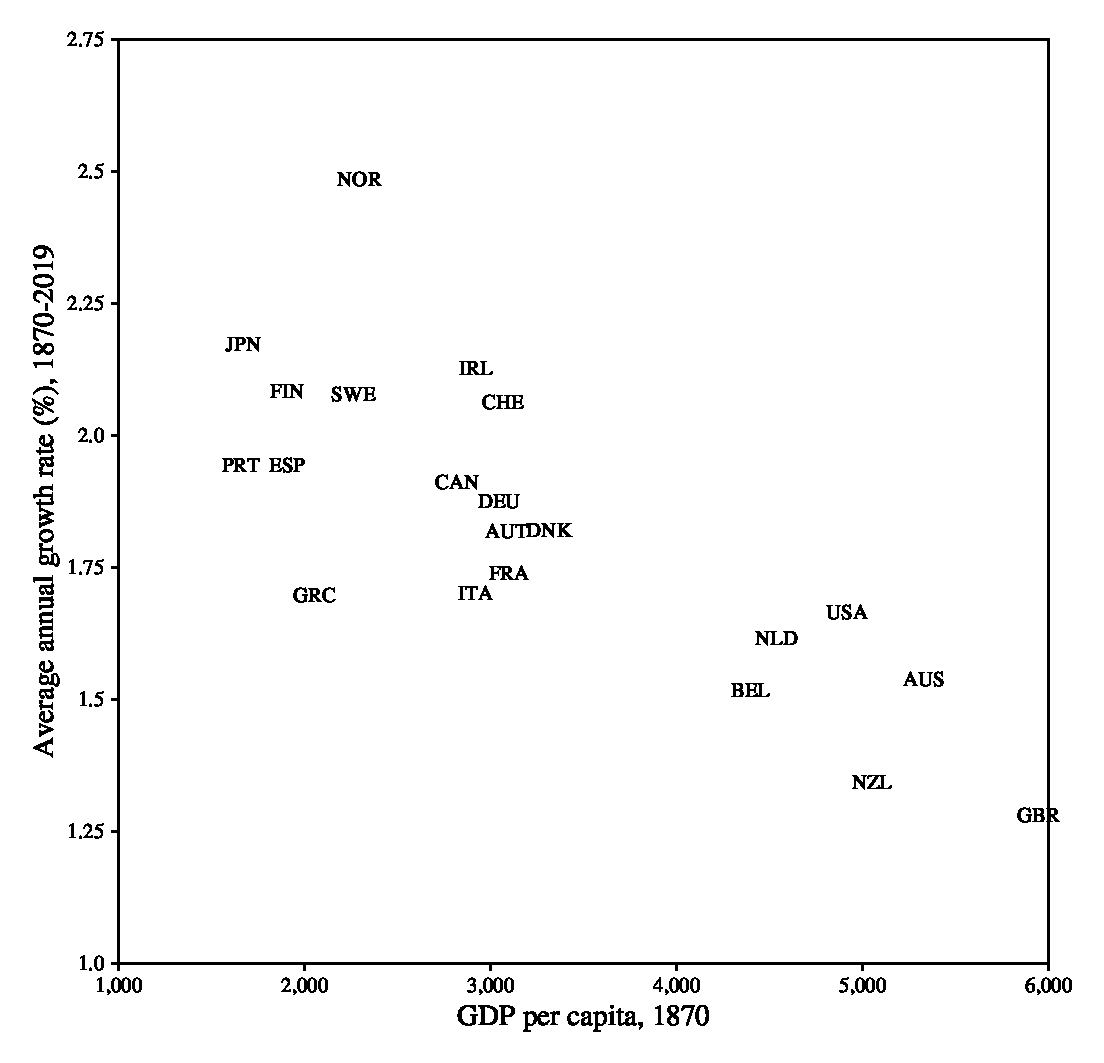
\includegraphics[height = 2.5in]{../Figures/fig-ch3-fig7.eps}
\end{center}
Why does this have to work? 
\end{frame}

\begin{frame}{Convergence in all countries}
But for countries in general it does not work
\begin{center}
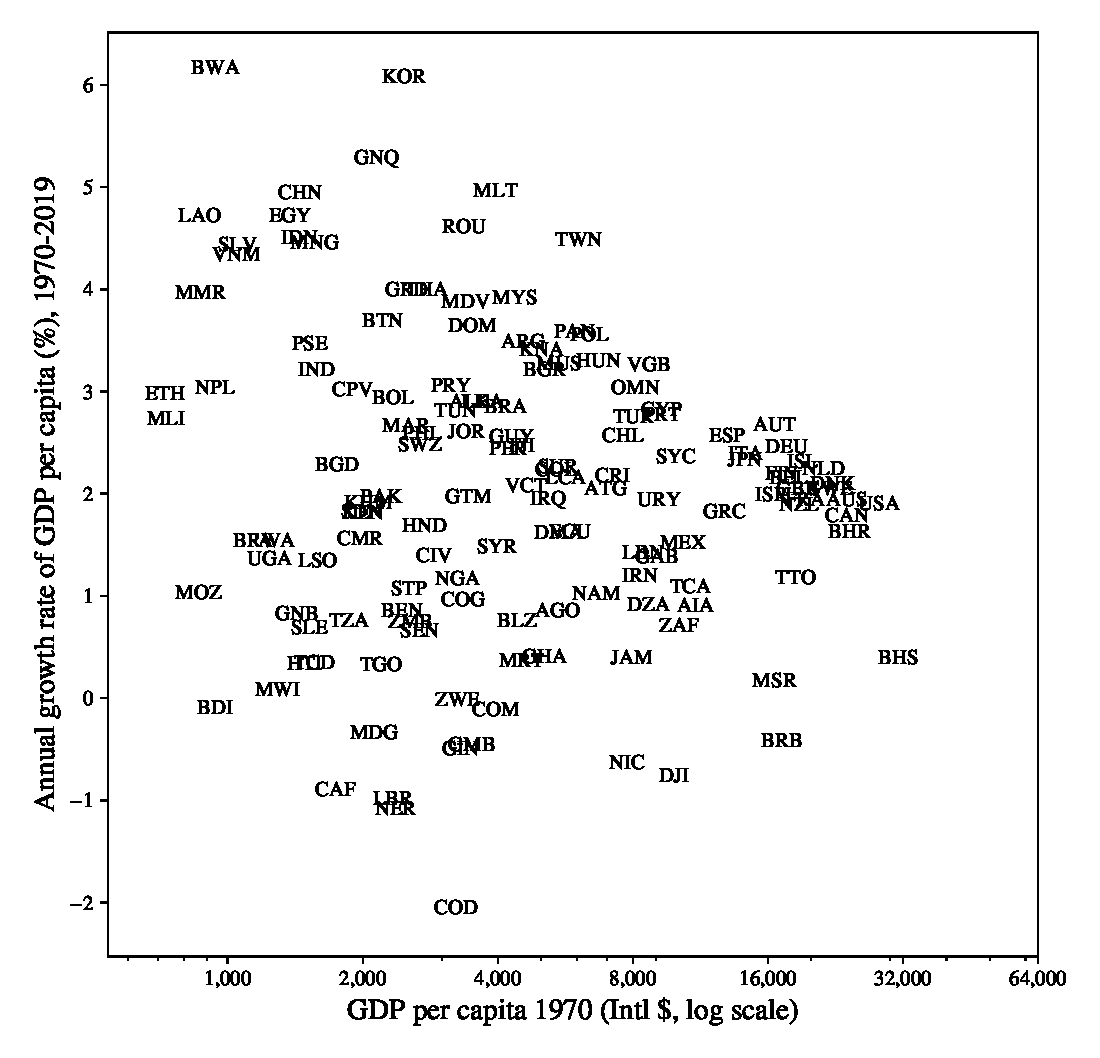
\includegraphics[height = 2.5in]{../Figures/fig-ch3-fig8.eps}
\end{center}
This doesn't work because steady states are different. Not everyone is headed to the same BGP.
\end{frame}

\begin{frame}{Conditional convergence}
But it does (kind of) work if we compare the growth rate of each country to how far from it's \textit{own} steady state they start out,
\begin{center}
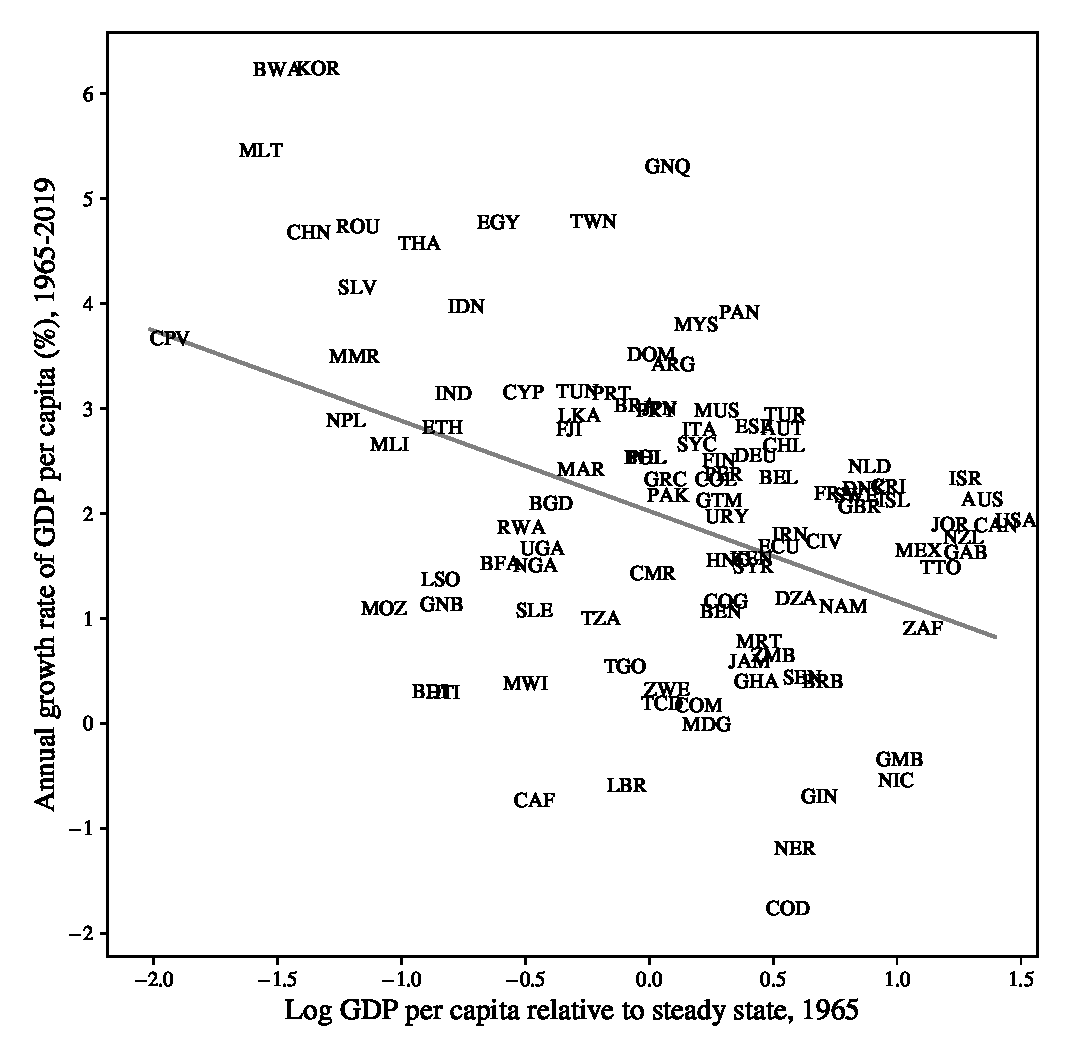
\includegraphics[height = 2.5in]{../Figures/fig-ch3-fig9.eps}
\end{center}
\end{frame}

\section{World Distribution}
\begin{frame}{How unequal is GDP per capita across countries?}
GDP per capita of the 90th to the 10th percentile
\begin{center}
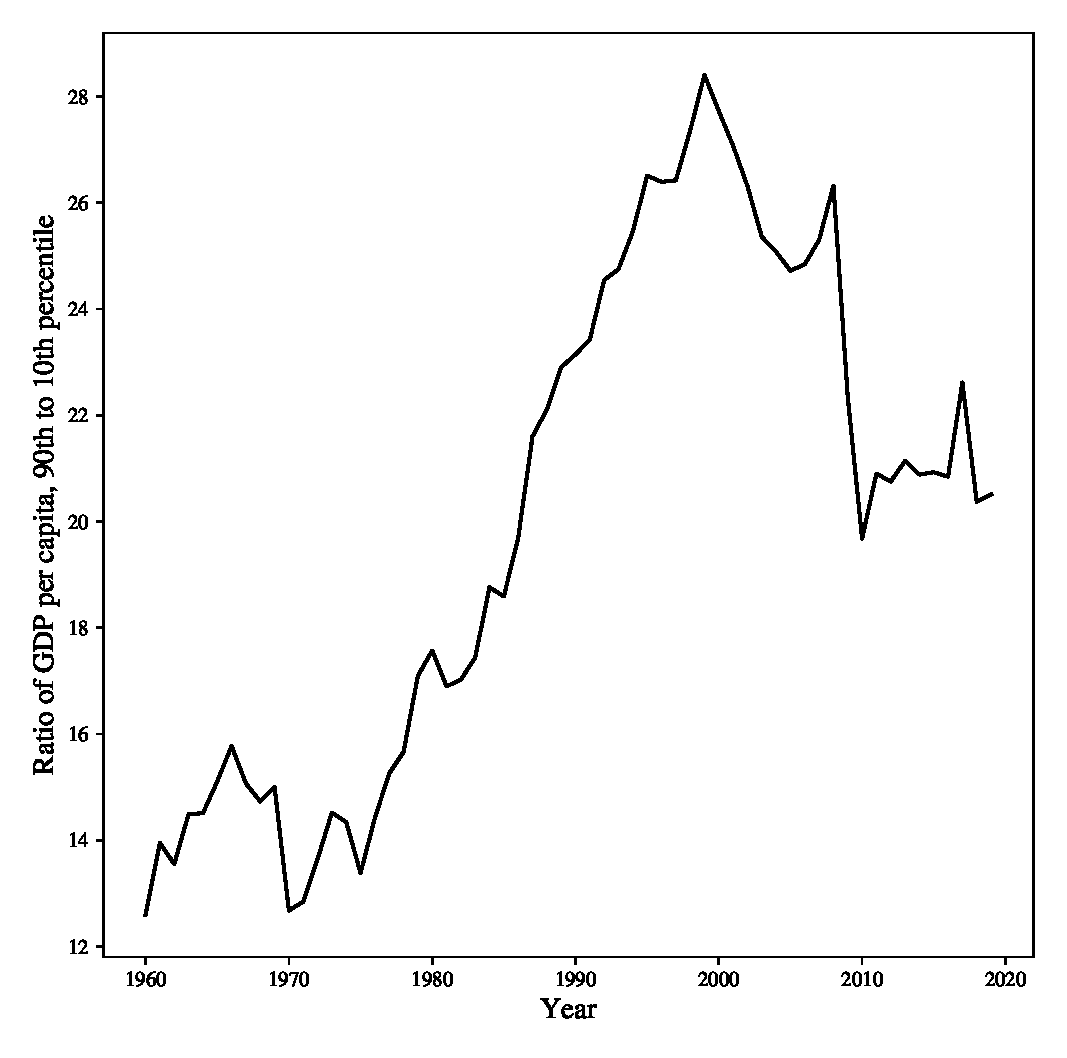
\includegraphics[height = 3in]{../Figures/fig-ch3-fig10.eps}
\end{center}
\end{frame}

\begin{frame}{How much higher is GDP per capita in general?}
Number of people living at different levels of GDP per capita
\begin{center}
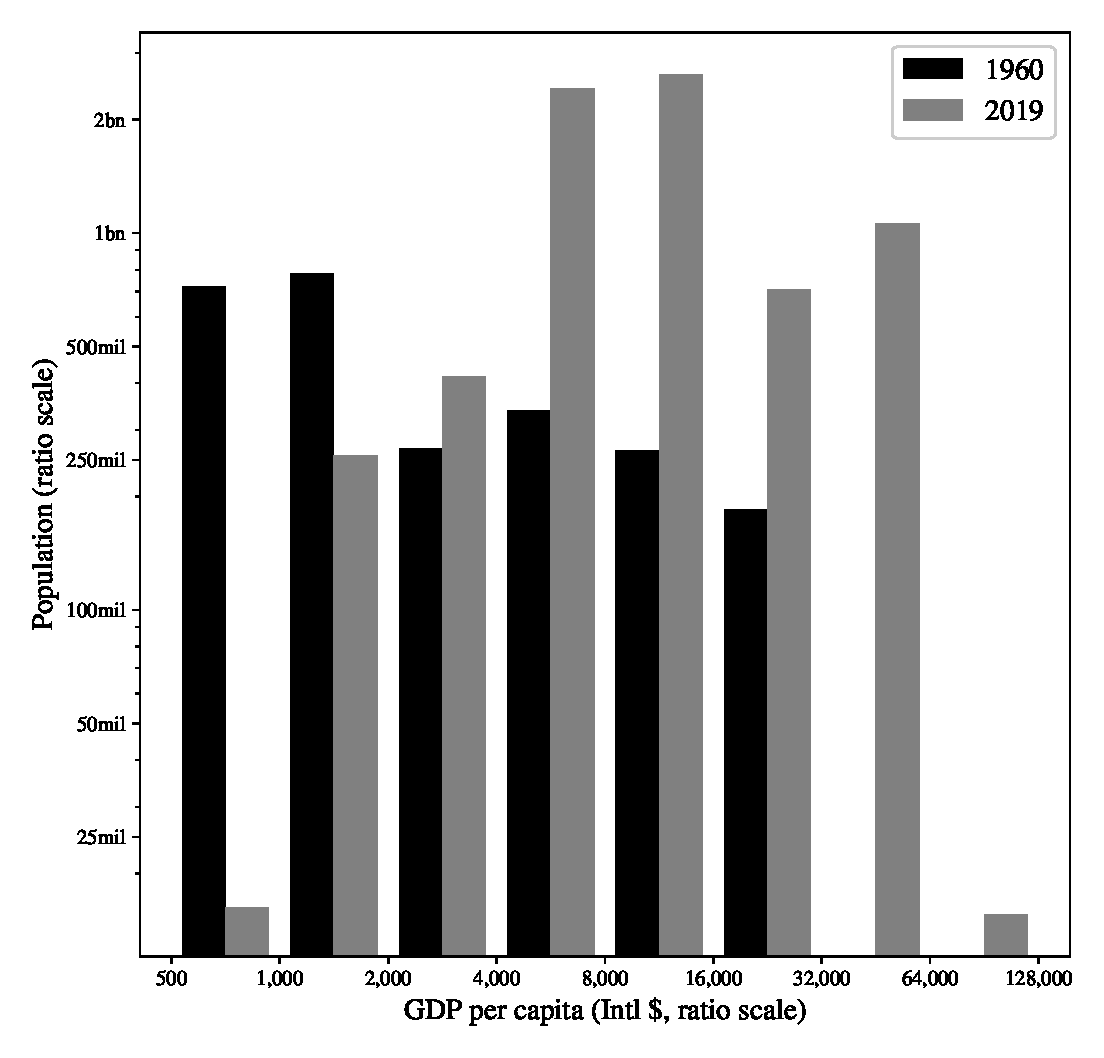
\includegraphics[height = 3in]{../Figures/fig-ch3-fig11.eps}
\end{center}
\end{frame}

\begin{frame}{How many people live in absolute poverty?}
Number of People Living in or out of Extreme Poverty, 1820-2015
\begin{center}
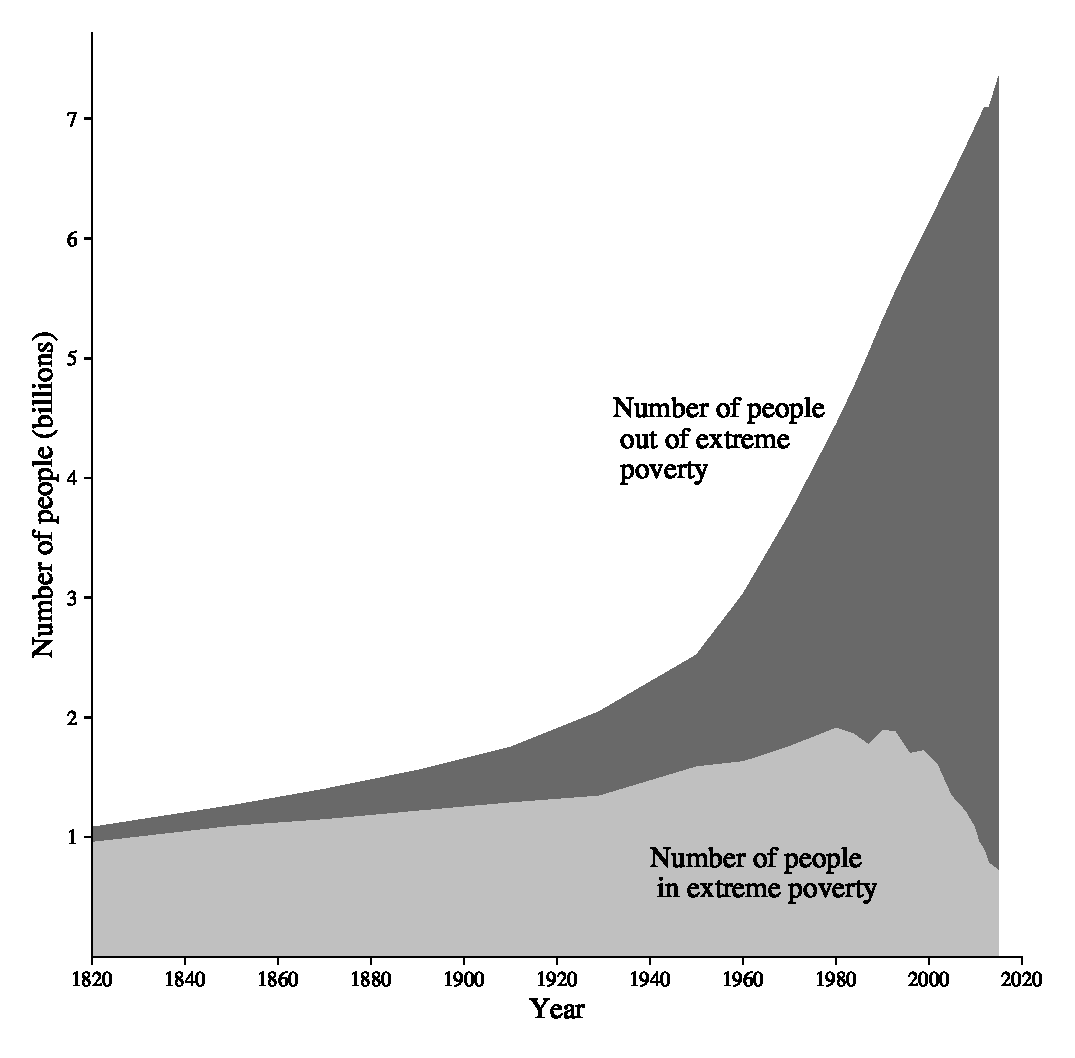
\includegraphics[height = 3in]{../Figures/fig-ch3-fig12.eps}
\end{center}
\end{frame}

\section{Accounting}
\begin{frame}{What drives growth?}
Growth is a combination of transitory growth and long-run growth:
\begin{equation}
	g_y = \underset{\text{Transitory}}{\alpha (g_K - g_A - g_L)} + \underset{\text{Long-run}}{g_A} \label{EQ_gy} \nonumber
\end{equation}
\begin{itemize}
	\item We can put numbers of each term
	\item Assume $\alpha = 0.3$
	\item We can measure, $g_y$, $g_K$, and $g_L$
	\item We can infer $g_A$ from the equation; it has to hold
\end{itemize}
\end{frame}

\begin{frame}{Accounting for the U.S.}
\begin{scriptsize}
\begin{center}
\begin{tabularx}{\textwidth}{lXXXXXX}
\midrule
               & \multicolumn{6}{c}{Growth rate (in percent):} \\ \cmidrule(lr){2-7}
        & 1955-1965 & 1965-1975 & 1975-1985 & 1985-1995 & 1995-2005 & 2005-2015 \\
Annualized growth: & (1)       & (2)       & (3)       & (4)       & (5)       & (6)    \\
\midrule
%\input{tab_ch3_tab1.txt}
\multicolumn{7}{c}{United States} \\
GDP per capita ($g_y$) & 2.15 & 2.04 & 2.49 & 1.93 & 2.32 & 0.72\\
\\
\multicolumn{7}{l}{Breakdown of GDP per capita growth:} \\
Productivity ($g_A$) & 2.25 & 1.90 & 2.73 & 2.10 & 2.59 & 0.75\\
Transitory ($\alpha (g_K - g_A - g_L)$) & -0.10 & 0.15 & -0.24 & -0.17 & -0.28 & -0.03\\
\\
\multicolumn{7}{l}{Breakdown of transitory growth:} \\
Capital ($g_K$) & 3.50 & 3.37 & 2.88 & 2.51 & 2.74 & 1.48\\
Productivity ($g_A$) & 2.25 & 1.90 & 2.73 & 2.10 & 2.59 & 0.75\\
Labor ($g_L$) & 1.58 & 0.99 & 0.93 & 0.98 & 1.07 & 0.84\\

\midrule
\end{tabularx}
\end{center}
\end{scriptsize}
\end{frame}

\begin{frame}{Accounting for Japan}
\begin{scriptsize}
\begin{center}
\begin{tabularx}{\textwidth}{lXXXXXX}
\midrule
               & \multicolumn{6}{c}{Growth rate (in percent):} \\ \cmidrule(lr){2-7}
        & 1955-1965 & 1965-1975 & 1975-1985 & 1985-1995 & 1995-2005 & 2005-2015 \\
Annualized growth: & (1)       & (2)       & (3)       & (4)       & (5)       & (6)    \\
\midrule
%\input{tab_ch3_tab1.txt}
\multicolumn{7}{c}{Japan} \\
GDP per capita ($g_y$) & 7.64 & 6.25 & 3.37 & 2.77 & 0.98 & 0.57\\
\\
\multicolumn{7}{l}{Breakdown of GDP per capita growth:} \\
Productivity ($g_A$) & 7.57 & 4.75 & 2.89 & 2.40 & 0.83 & 0.75\\
Transitory ($\alpha (g_K - g_A - g_L)$) & 0.08 & 1.50 & 0.48 & 0.38 & 0.15 & -0.18\\
\\
\multicolumn{7}{l}{Breakdown of transitory growth:} \\
Capital ($g_K$) & 8.79 & 10.99 & 5.31 & 4.02 & 1.48 & 0.12\\
Productivity ($g_A$) & 7.57 & 4.75 & 2.89 & 2.40 & 0.83 & 0.75\\
Labor ($g_L$) & 0.96 & 1.23 & 0.81 & 0.36 & 0.15 & -0.03\\

\midrule
\end{tabularx}
\end{center}
\end{scriptsize}
\end{frame}

\begin{frame}{What drives growth?}
What do we learn?
\begin{itemize}
	\item Even for Japan, which had a big transition to a higher BGP, capital accumulation and transitory growth was relatively small
	\item Some of what happened was that $A_0$ kept going up, so there was some transition in the level of productivity
	\item Ultimately the growth rate of productivity is important for long-run growth
	\item Capital accumulation and transition are relevant for catching up
	\item We need to study productivity levels and growth in detail
\end{itemize}
\end{frame}


\end{document}